\documentclass[mirror]{revdetua}
%
% Valid options are:
%   portugues --------- main language is Portuguese
%   final ------------- final version (default)
%   times ------------- use times (postscript) fonts for text
%   mirror ------------ prints a mirror image of the paper (with dvips)
%   visiblelabels ----- \SL, \SN, \SP, \EL, \EN, etc. defined
%   invisiblelabels --- \SL, \SN, \SP, \EL, \EN, etc. not defined (default)
%
% Note: the final version should use the times fonts
% Note: the really final version should also use the mirror option
%

\usepackage[portuguese]{babel}
\usepackage[utf8]{inputenc}
\usepackage{amsmath} 
\usepackage{comment}
\usepackage{algorithm}
\usepackage{algpseudocode}
\usepackage{graphicx}
\usepackage[justification=centering]{caption}
\floatname{algorithm}{Algoritmo}
%-------------------------------------
% compiling:
% Recipe: xelatex
% Recipe: pdflatex -> bibtex -> pdflatex -> pdflatex
% Recipe: xelatex
%-------------------------------------
\begin{document}

\Header{01}{01}{Novembro}{2024}{1}

\title{Maximum Weight Cut}
\author{Hugo Veríssimo - 124348 - hugoverissimo@ua.pt}
\maketitle

\begin{abstract}
This report presents the implementation and comparison of two methods for solving the Max Weight Cut problem: an exhaustive search and a greedy heuristic. The Max Weight Cut problem consists of dividing a graph into two complementary subsets in order to maximize the sum of the weights of the edges that connect the two subsets. While exhaustive search guarantees an optimal solution, its computational complexity makes it impractical for large graphs. On the other hand, the greedy heuristic provides fast solutions, although suboptimal ones. The experimental results demonstrate the trade-off between accuracy and performance, highlighting the efficiency of the heuristic for graphs with a larger number of vertices.
\end{abstract}

\begin{resumo}
Este relatório apresenta a implementação e comparação de dois métodos para resolver o problema \textit{Max Weight Cut}: uma pesquisa exaustiva e uma heurística gulosa. O problema \textit{Max Weight Cut} consiste em dividir um grafo em dois subconjuntos complementares, de forma a maximizar a soma dos pesos das arestas que ligam os dois subconjuntos. Enquanto a pesquisa exaustiva garante uma solução ótima, a sua complexidade computacional torna-a impraticável para grafos de grande dimensão. Por outro lado, a heurística gulosa fornece soluções rápidas, embora subótimas. Os resultados experimentais demonstram o compromisso entre precisão e desempenho, destacando a eficiência da heurística para grafos com maior número de vértices.
\end{resumo}

\section{Introdução}

Atualmente, os problemas em grafos são amplamente estudados, pelo facto de terem a capacidade de modelar diversas situações reais, desde as mais palpáveis, como redes de computadores (problema \textit{Minimum Spanning Tree}) até às mais abstratas, como física estatística (problema \textit{Maximum Weight Cut}) \cite{WANG10}.

Este relatório visa explorar o problema \textit{Maximum Weight Cut}, conhecido em português por Corte de Peso Máximo, que consiste na divisão de um grafo não direcionado, $G(V, E)$, onde $|V| = n$ vértices e $|E| = m$ arestas de peso $w_{i,j} \geq 0\ \forall\ (i,j) \in E$, em dois subconjuntos complementares, $S$ e $T$, de forma a maximizar a soma dos pesos das arestas que ligam os dois conjuntos \cite{SC03}, isto é
\begin{equation*}
    \begin{split}
        \max \sum_{i \in S,\ j \in T} w_{i,j} \\ 
        \left\{\begin{split}
            &S \cup T = V \\
            &S \cap T = \emptyset
        \end{split}\right.
    \end{split}
\end{equation*}

Apesar do problema oposto, conhecido como \textit{Minimum Weight Cut}, ter um algoritmo de resolução em tempo polinomial, em certas condições, o problema \textit{Maximum Weight Cut} não o possui, sendo um problema \textit{NP-Hard}. Isto implica que à medida que o tamanho do grafo aumenta, encontrar soluções exatas para este problema tornam-se computacionalmente caras \cite{SS23}.

Ao longo deste relatório, serão abordadas duas estratégias para a resolução do problema: uma pesquisa exaustiva e uma heurística gulosa.

% pode se meter aqui foto la do problema

\section{Metodologia da Análise}

Com o intuito de analisar o problema em destaque, foi utilizada a linguagem de programação \textit{Python}, conhecida pela sua simplicidade e pela vasta variedade de bibliotecas, tais como \textit{networkx}, \textit{numpy} e \textit{itertools}, que facilitaram a implementação das estratégias propostas.

A análise desenvolvida pode ser dividida em 2 ficheiros principais, sem desmerecer o uso de ficheiros auxiliares, sendo os primeiros:
\begin{verbatim}
    $ python3 graphs.py
    $ python3 benchmarks.py
\end{verbatim}

O ficheiro \textit{graphs.py} teve como propósito gerar vários grafos aleatórios, tendo em conta a semente 124348, com diferentes número de vértices, número de arestas e peso de arestas, de forma a avaliar o comportamento das estratégias aplicadas em diferentes cenários.

O ficheiro \textit{benchmarks.py} foi o responsável por executar as estratégias de resolução do problema, nomeadamente a pesquisa exaustiva e a heurística gulosa, para vários grafos gerados, guardando os resultados obtidos, tais como tempo de execução, número de operações básicas e precisão do resultado da heurística gulosa, para posterior análise.

%meter imagem de um dos grafos com nome na fig e isso?

\section{Algoritmo de Pesquisa Exaustiva}

Tendo em conta o algoritmo de pesquisa exaustiva, este visa gerar todas as combinações possíveis de subconjuntos de $V$ e, para cada subconjunto, calcular o peso do corte e comparar com o melhor corte encontrado até ao momento, ou seja, o algoritmo tem duas fases: a geração de todos os subconjuntos possíveis e a avaliação de cada subconjunto. Este estratégia garante a obtenção da solução ótima, no entanto, o seu custo computacional é exponencial, sendo impraticável para grafos de grande dimensão. Este algoritmo pode ser representado em pseudocódigo da seguinte maneira:

\begin{algorithm}
    \raggedright
    \textbf{Entrada:} matriz de adjacência \textit{G} \\
    \textbf{Saída:} subconjuntos \textit{S} e \textit{T}, peso do corte \textit{weight} \\
    \hrule 
    \caption{Pesquisa Exaustiva}
    \begin{algorithmic}[1]
        \State input\_set $\gets$ \{0, 1, \ldots, \text{len(G)} - 1\}
        \State subsets $\gets$ \text{EMPTY LIST}
        \State n $\gets$ \text{LENGTH OF input\_set}
        
        \Comment{Generate all subsets}
        \For{r from 0 to n}
            \For{each S in combinations(input\_set, r)}
            \State Add S to subsets
            \EndFor
        \EndFor
        
        \State best $\gets$ input\_set
        \State weight $\gets$ 0
        
        \Comment{Evaluate each subset}
        \For{each S in subsets}
            \State new\_weight $\gets$ 0
            \For{each i in S}
                \For{each j in input\_set - S}
                    \State new\_weight $\gets$ new\_weight + G[i, j]
                \EndFor
            \EndFor
            
            \If{new\_weight $>$ weight}
            \State best $\gets$ S
            \State weight $\gets$ new\_weight
            \EndIf
        \EndFor
        \State S $\gets$ best
        \State T $\gets$ input\_set - best
        \State \Return S, T, weight
    \end{algorithmic}
\end{algorithm}


Pode-se verificar que as duas fases deste algoritmo apresentam complexidades $O(2^n)$ e $O(2^n \times n^2)$, respetivamente. A primeira devido ao processo de geração de todos os subconjuntos possíveis ($2^n$) e a segunda devido ao processo de percorrer cada subconjunto ($2^n$) e para cada qual percorrer todas as combinações de arestas, mesmo com peso $0$, entre o próprio e o seu complementar (no pior caso, $(n \div 2)^2 \rightarrow n^2$).

Assim, verifica-se que a complexidade deste algoritmo é exponencial com um fator polinomial: $O(2^n \times n^2)$, o que reforça a ideia de que este algoritmo é impraticável para grafos de grande dimensão, daí a necessidade de algoritmos alternativos, como o algoritmo de pesquisa gulosa.


\section{Algoritmo de Pesquisa Gulosa}

Atendendo ao algoritmo de pesquisa gulosa com heurísticas, este segue uma abordagem diferente, uma vez que não garante a obtenção da solução ótima, mas sim uma solução aproximada, em tempo polinomial. Isto acontece devido à natureza do algoritmo, que em cada etapa faz escolhas localmente ótimas, sem considerar o impacto global da escolha, na esperança de alcançar um ótimo global.

Para o desenvolvimento este algoritmo, foi necessária uma análise a diversas regras heurísticas \cite{WANG23}, com o objetivo de determinar a melhor estratégia a seguir. Desta forma, a estratégia escolhida pode ser examinada em detalhe no pseudocódigo apresentado a seguir.

\begin{algorithm}
    \raggedright
    \textbf{Entrada:} matriz de adjacência \textit{G} \\
    \textbf{Saída:} subconjuntos \textit{S} e \textit{T}, peso do corte \textit{cut\_weight} \\
    \hrule 
    \caption{Pesquisa Gulosa}
    \begin{algorithmic}[1]
    
        \State n $\gets$ \text{len}(G)

        \Comment{Extract edges and their weights}
        \State edges $\gets$ \text{EMPTY LIST}
        \For{i from 0 to n - 1}
            \For{j from i + 1 to n - 1}
                \State weight $\gets G[i, j]$
                \State Add (i, j, weight) to edges
            \EndFor
        \EndFor

        \State Sort edges in descending order by weight

        \Comment{Process each edge}
        \State cut\_weight $\gets$ 0
        \State seen, S, T $\gets$ \text{EMPTY SETS}
        \For{each (u, v, weight) in edges}
            \If{u not in seen and v not in seen}
                \State cut\_weight $\gets$ cut\_weight + weight
                \State Add u to S, add v to T
                \State Update seen with \{u, v\}
            \ElsIf{u in S and v not in seen}
                \State cut\_weight $\gets$ cut\_weight + weight
                \State Add v to T, add v to seen
            \ElsIf{u in T and v not in seen}
                \State cut\_weight $\gets$ cut\_weight + weight
                \State Add v to S, add v to seen
            \ElsIf{v in S and u not in seen}
                \State cut\_weight $\gets$ cut\_weight + weight
                \State Add u to T, add u to seen
            \ElsIf{v in T and u not in seen}
                \State cut\_weight $\gets$ cut\_weight + weight
                \State Add u to S, add u to seen
            \ElsIf{u in S and v in T}
                \State cut\_weight $\gets$ cut\_weight + weight
            \ElsIf{v in S and u in T}
            \State cut\_weight $\gets$ cut\_weight + weight
            \Else
                \Comment{Both u and v have been seen, skip}
            \EndIf
        \EndFor

        \State \Return S, T, cut\_weight
    
    \end{algorithmic}
\end{algorithm}

%\pagebreak
% pq texto estava a ficar antes do alg para ter mais texto idk why cuidado

Pode-se observar que o algortimo tem duas etapas: uma de pré-processamento, onde são extraídas as arestas e os seus pesos e ordenados de forma decrescente, e outra de processamento, onde as arestas são processadas de acordo com as regras heurísticas definidas.

A primeira etapa deste algoritmo é a mais custosa em termos de complexidade, sendo $O(n^2 + m \log m)$. Sendo que o grafo tem no total $0.5 \cdot n(n-1)$ arestas, contabilizando as nulas, o termo $m \log m$ torna-se dominante, pelo que a complexidade da etapa possa ser escrita como $O(n^2 \log n)$.

A segunda etapa, por sua vez, tem uma complexidade $O(m)$, dado que que percorre todas as arestas do grafo, nulas inclusive, podendo ser escrita como $O(n^2)$.

Portanto, pode-se concluir que esta abordagem apresenta uma complexidade polinomial com um fator logarítmico adicional: $O(n^2 \log n)$.

\section{Análise dos Resultados}

Após a implementação e execução dos algoritmos de pesquisa exaustiva e heurística gulosa, através do ficheiro \textit{benchmarks.py}, foi possível analisar os resultados obtidos, nomeadamente o número de operações básicas, o tempo de execução, a quantidade de diferentes soluções testadas e a precisão da solução da heurística gulosa.

\subsection{Análise do Número de Operações}

Pelo facto da complexidade de um algoritmo ser uma medida fundamental para compreender a sua eficiência, e a primeira poder ser medida em termos do número de operações básicas que ele realiza, em função do tamanho do parâmetro de entrada \cite{BS22}, esta análise visa validar as complexidades teóricas previamente discutidas nas secções referentes a cada algoritmo.

Para isso, é criado um gráfico que ilustra o número total de operações básicas executadas, por ambos os algoritmos, para grafos com diferentes números de arestas e de vértices.

\begin{figure}[h]
    \centering
    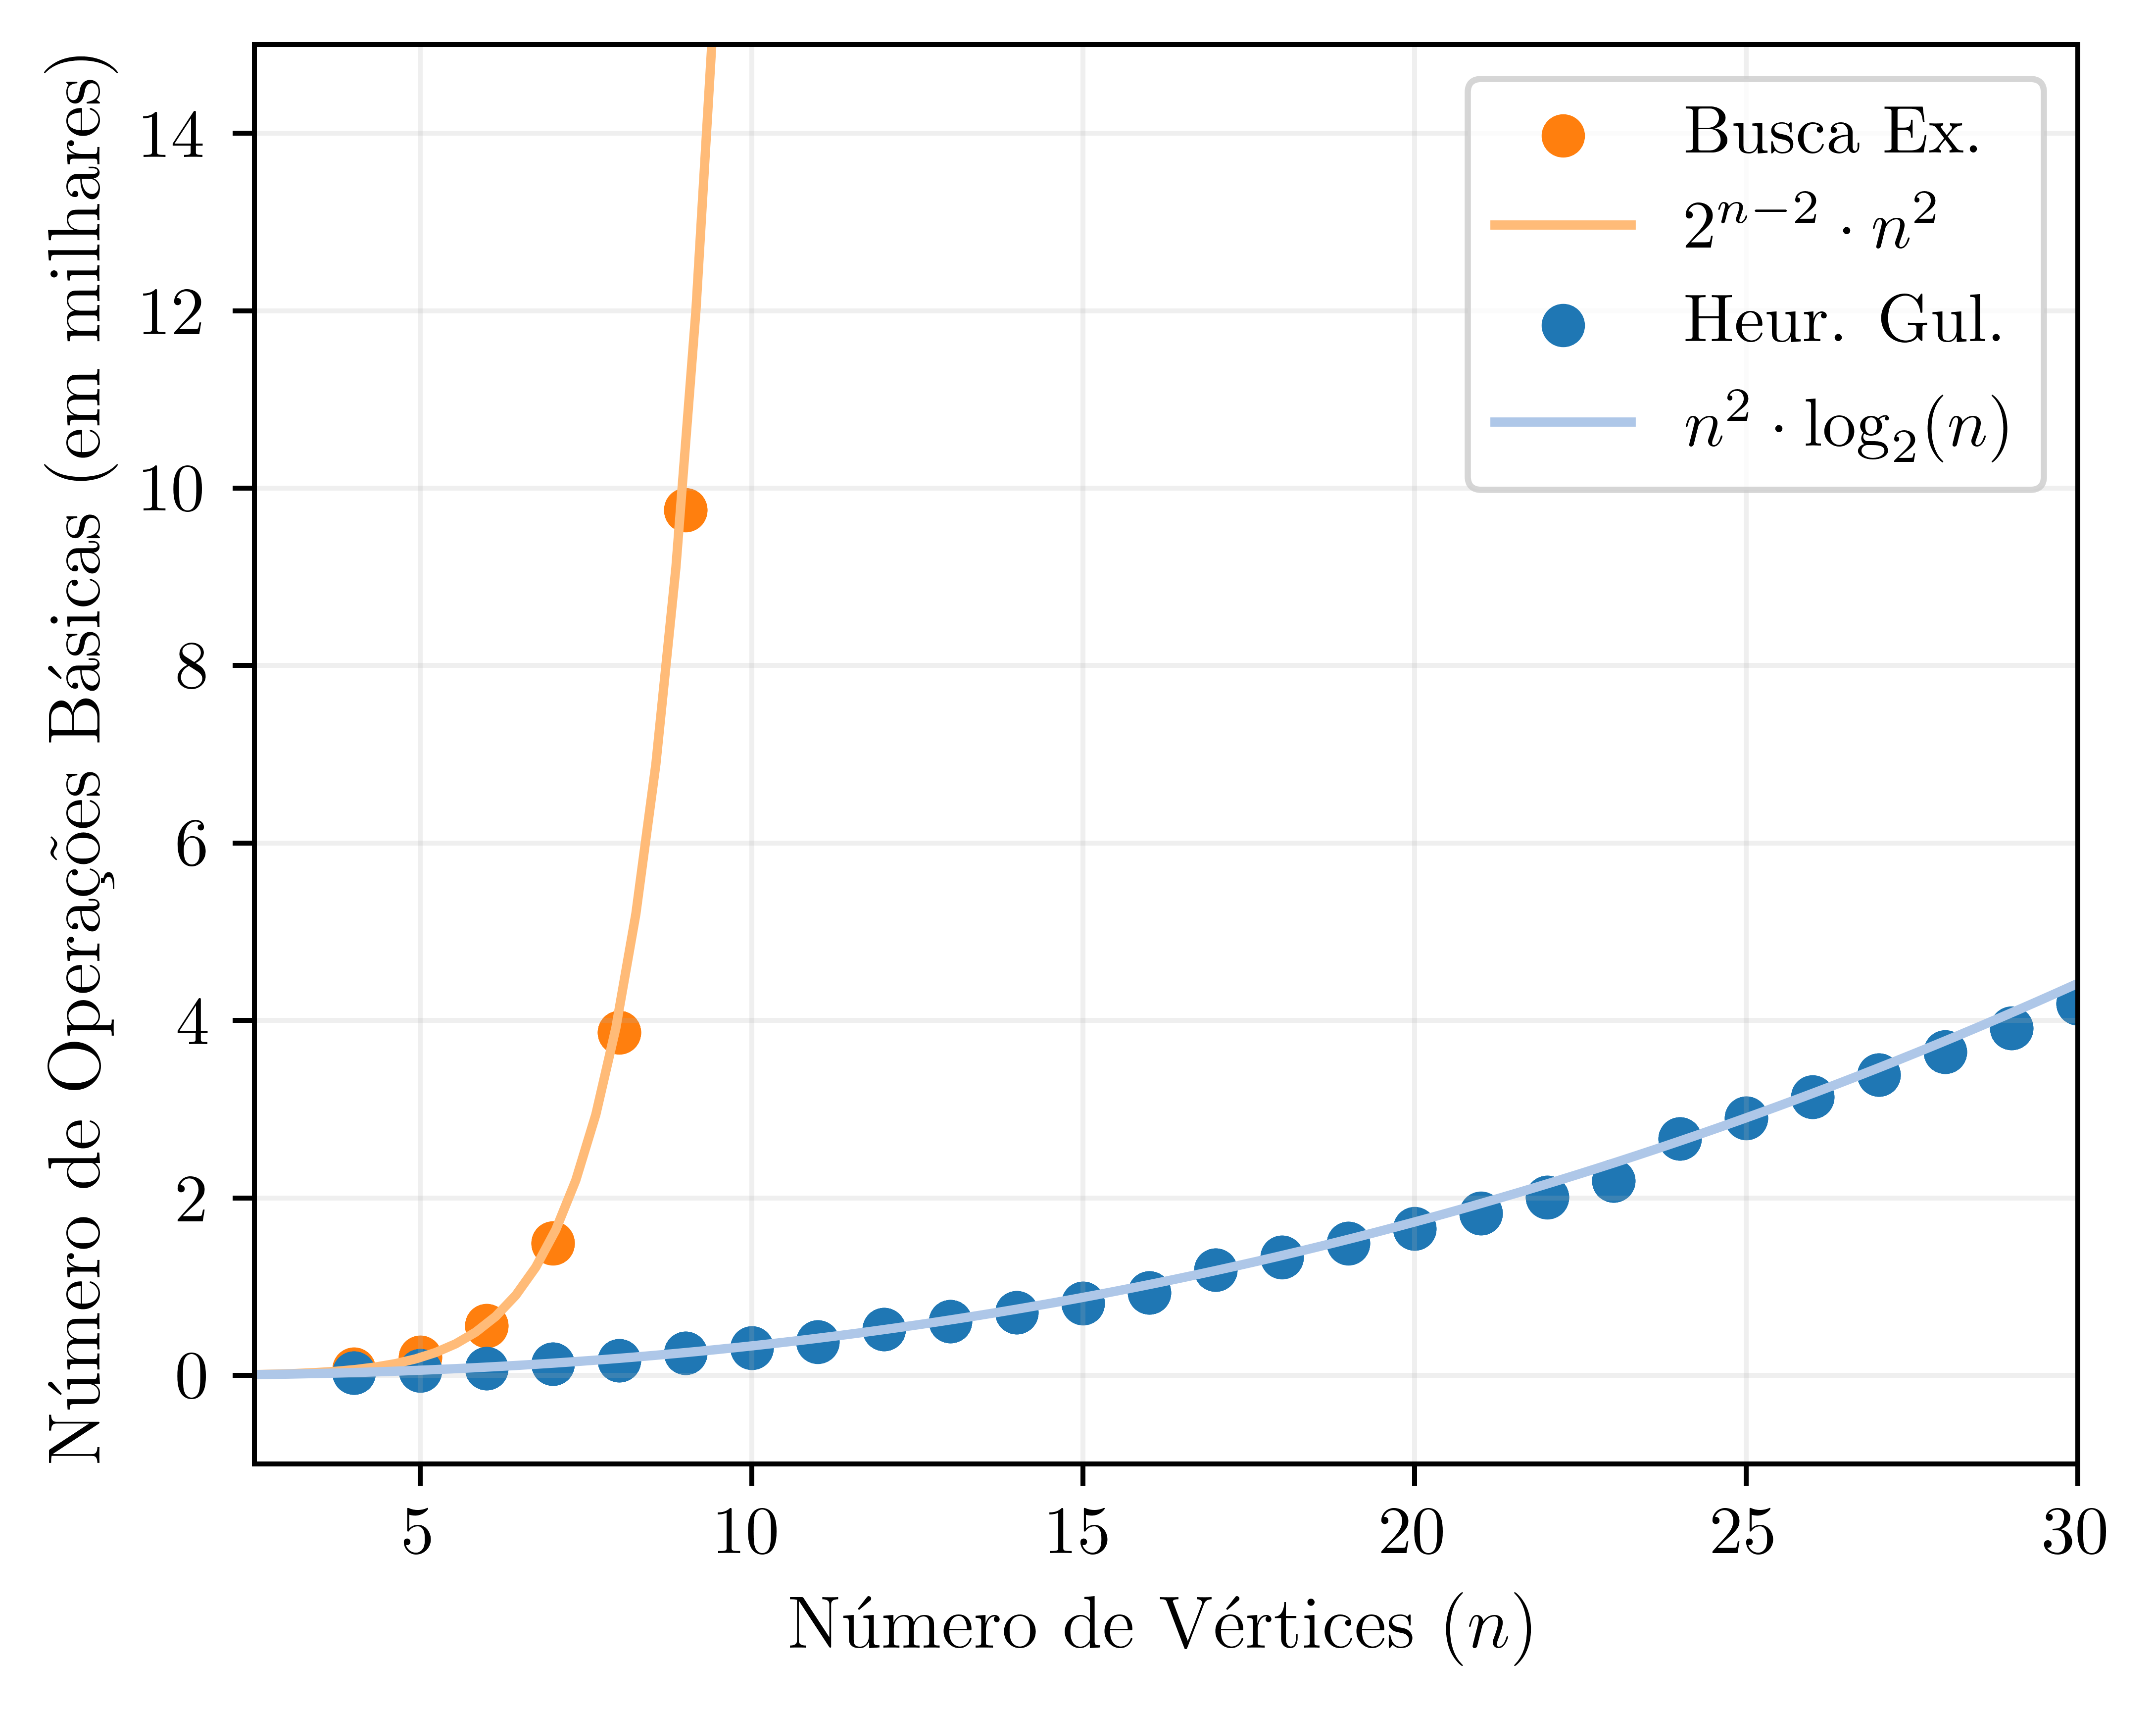
\includegraphics[width=0.4\textwidth]{../assets/numberOPS.png}
    \caption{Número de operações básicas realizadas pelos algoritmos de pesquisa exaustiva e heurística gulosa em função do número de vértices, para diferentes grafos.}
    \label{fig:numeroops}
\end{figure}

Pode-se observar no gráfico, a laranja, a informação relativa ao algoritmo de pesquisa exaustiva, especificamente, os resultados para diferentes grafos, representados por pontos, e uma linha que representa a função $e(n) = 2^{n-2} \times n^2$, que modela de forma eficaz o comportamento do número de operações realizadas por este algoritmo. Analogamente, a azul, encontra-se a informação relativa ao algoritmo de heurística gulosa, cujos resultados são modelados pela função $f(n) = n^2 \log n$.

Assim, é possível verificar que o número de operações básicas realizadas pelos algoritmos é consistente com as complexidades teóricas previamente referidas: $O(2^n \times n^2)$, para o algortimo de pesquisa exaustiva, e $O(n^2 \log n)$, para o algoritmo de heurística gulosa, reforçando a ideia de que a heurística gulosa é mais eficiente que a pesquisa exaustiva, em termos de complexidade.

Para além disso, é importante destacar que não há diferenças significativas no número de operações realizadas pelos algoritmos em relação ao número de arestas, o que é evidenciado no gráfico pelo facto de grafos com o mesmo número de vértices, mas com diferentes quantidades de arestas, estarem sobrepostos. Isto está relacionado com o facto de ambos os algoritmos analisarem todas as arestas possíveis, ao invés de apenas as arestas com peso diferente de zero, de forma a evitar possíveis problemas relacionados a nós soltos.


\subsection{Análise de Tempo de Execução}

Outra métrica relevante na avaliação de algoritmos é o tempo de execução, uma vez que permite compreender a eficiência das operações e do algoritmo em relação ao tamanho do parâmetro de entrada. Ademais, esta análise possibilita comparações objetivas entre diferentes abordagens, facilitando a escolha do algoritmo mais adequado de acordo com cada situação.

Contudo esta métrica pode ser facilmente influenciada por diversos fatores, tais como o ambiente em que o algoritmo é executado, nomeadamente as especificações do \textit{hardware} utilizado, e as características específicas dos grafos \cite{NP15}. Para minimizar a risco do enviesamento destes resultados, foram realizadas pelo menos três medições para cada grafo, tendo sido escolhido o tempo mínimo entre elas, para ter uma maior coerência nos dados obtidos. Para além disso, todas as execuções foram realizadas num \textit{MacBook Air}, com um processador \textit{Apple M1} e $16GB$ de memória RAM, garantindo a manutenção de um \textit{hardware} constante para a análise.

Assim, para a realização desta análise, foi criado um gráfico que ilustra o tempo de execução de cada algoritmo, para diferentes grafos, em função do número de vértices.

\begin{figure}[h]
    \centering
    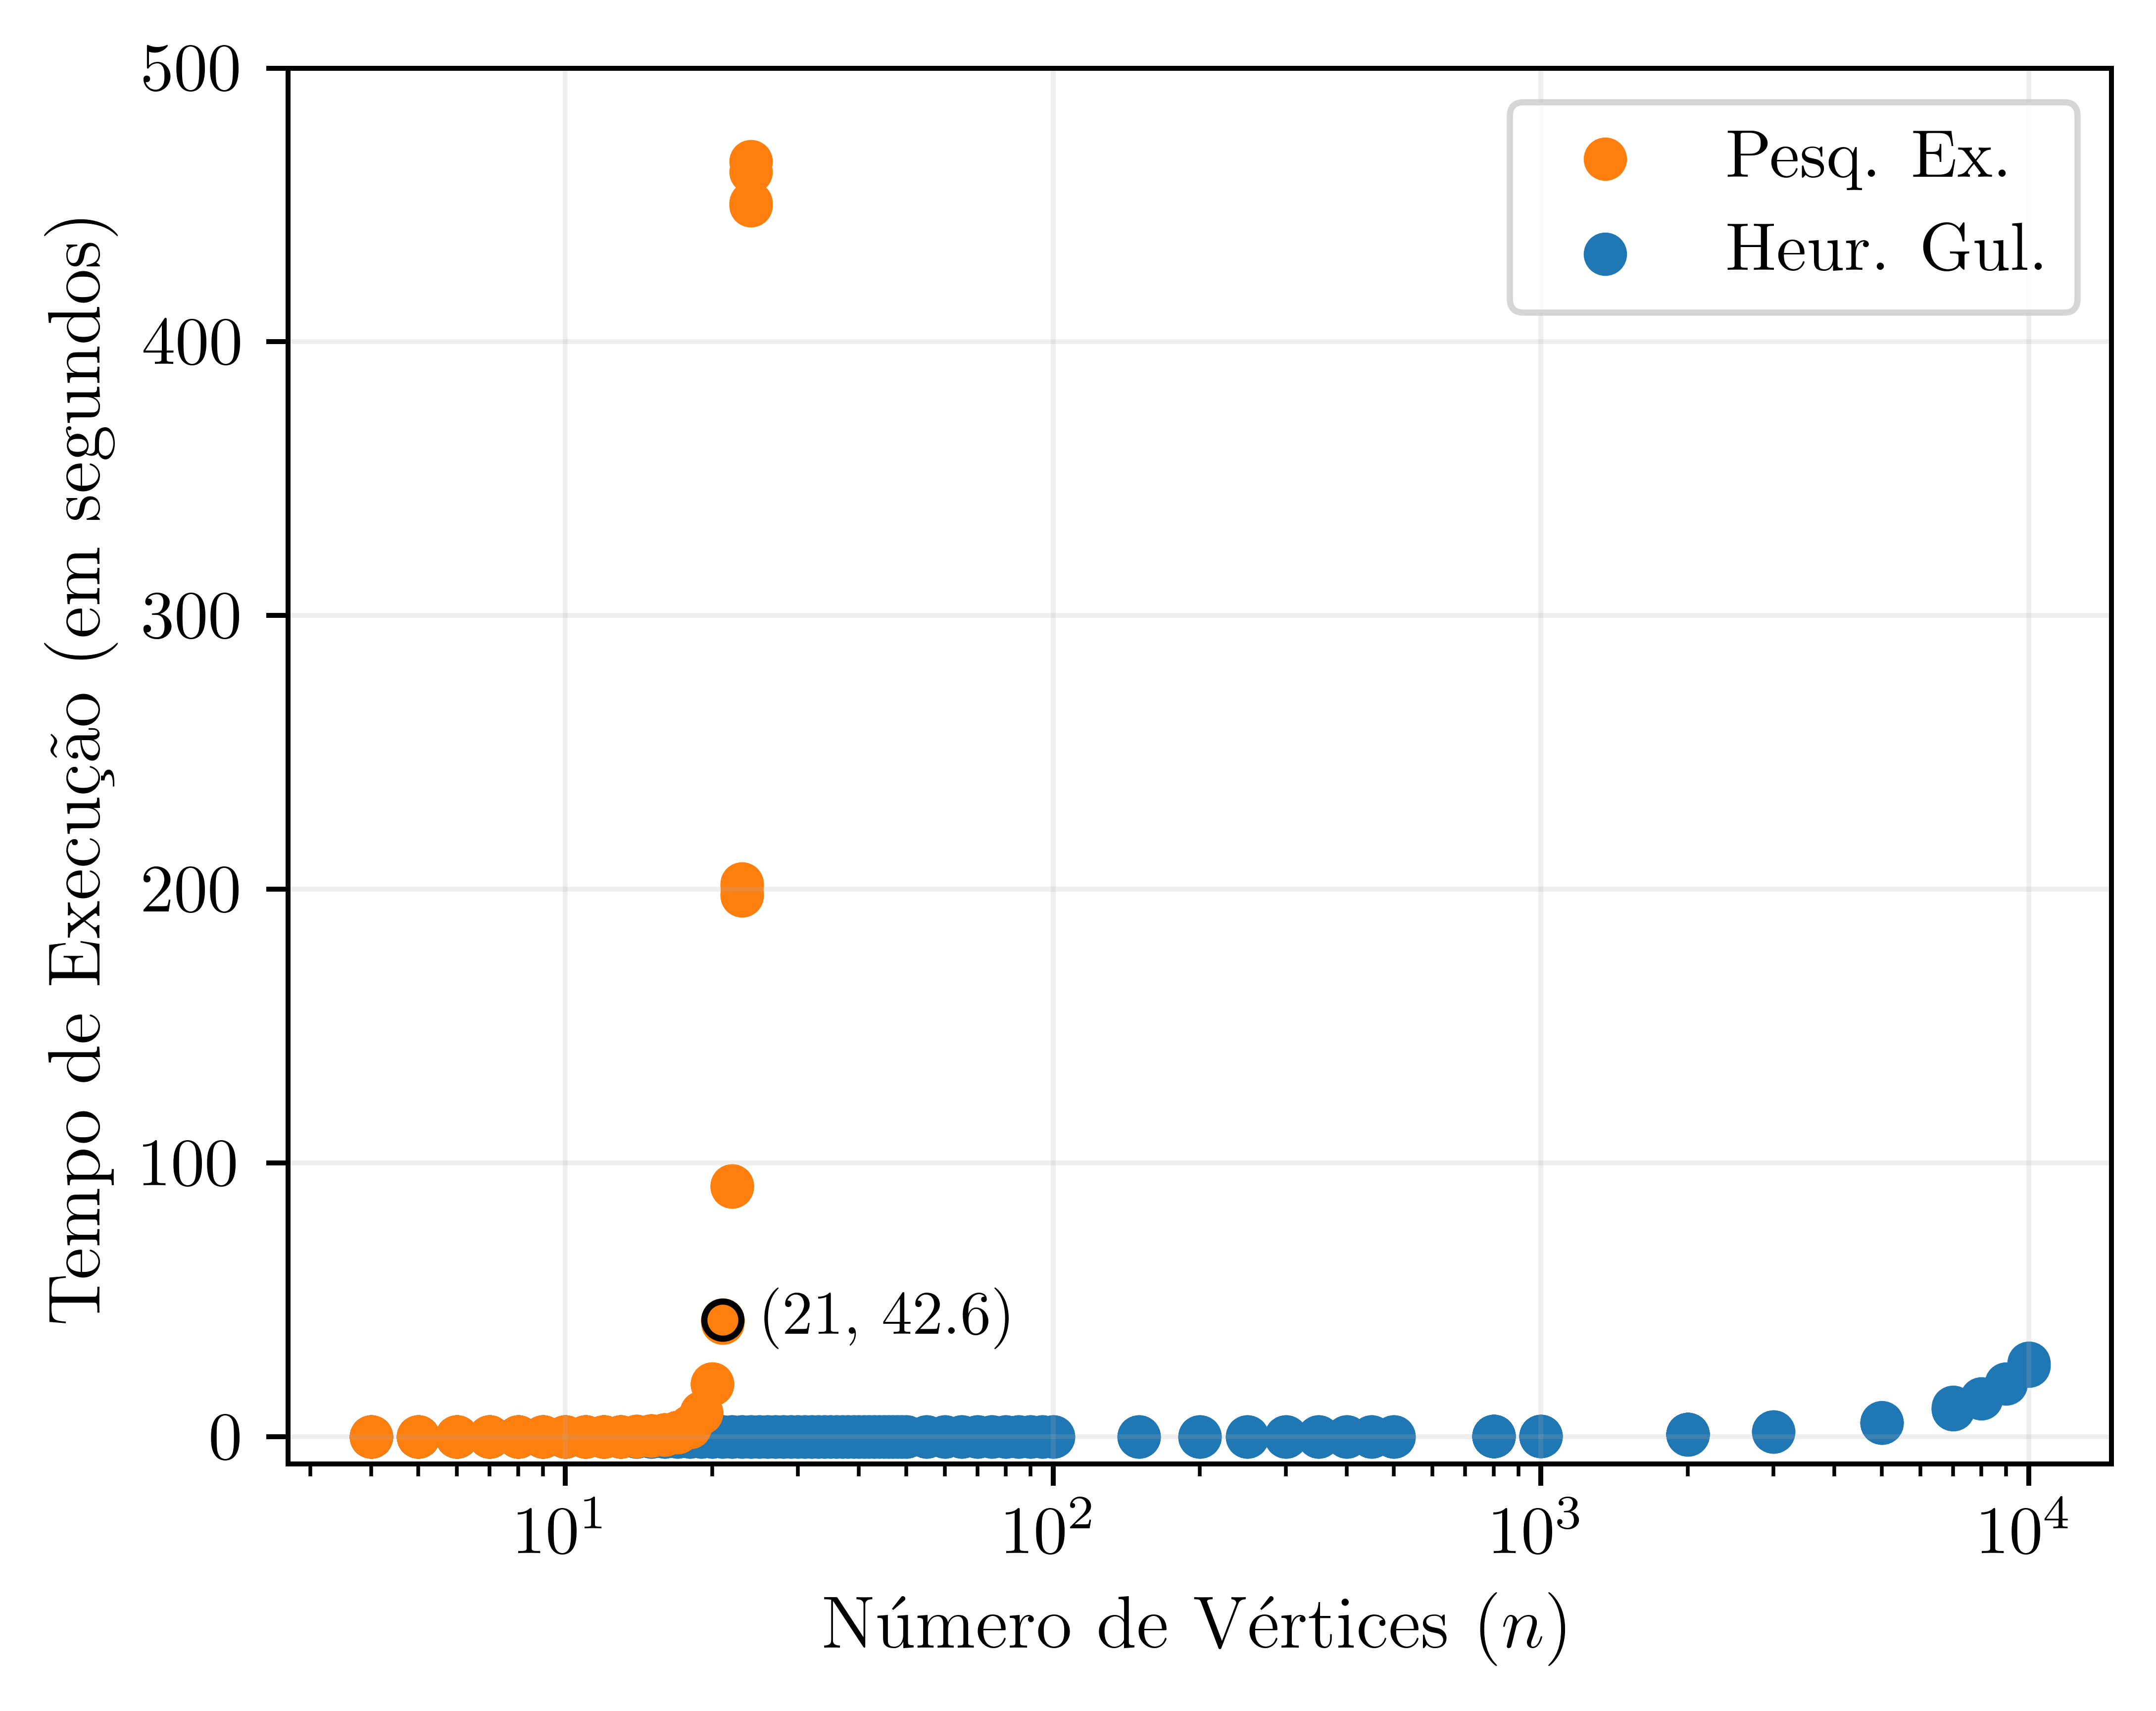
\includegraphics[width=0.4\textwidth]{../assets/execTIME.png}
    \caption{Tempo de execução dos algoritmos de pesquisa exaustiva e heurística gulosa em função do número de vértices, para diferentes grafos.}
    \label{fig:exectime}
\end{figure}

A partir do gráfico, é possível verificar os tempos de execução, em função do número de vértices para o algoritmo de pesquisa exaustiva, a laranja, e para o algoritmo de heurística gulosa, a azul. 

Atendendo ao algoritmo de pesquisa exaustiva, é possível reparar que a partir de $n = 21$, o tempo de execução explode, sendo mais notório o comportamento exponencial do algoritmo. Por outro lado, como seria de esperar, o algoritmo de heurística gulosa apenas apresenta o seu crescimento quadrático, de forma mais notória, a partir de $n \approx 10^4$, revelando-se significativamente mais eficiente que o algoritmo de pesquisa exaustiva em grafos de maiores dimensões.

De modo a prever o tempo de execução para grafos de maior dimensão, foram ajustadas regressões para os tempos de execução de cada algoritmo, de modo a obter funções que modelassem o comportamento dos mesmos. O critério usado para a modelação foi a minimização da medida de erro \textit{Normalized Mean Absolute Error} (NMAE).

% Justificação do Termo Exponencial na pesquisa Exaustiva e q retas foram usadas e tudo mais e pq q deu assim

Assim, obteve-se que o tempo de execução do algoritmo de pesquisa exaustiva pode ser modelado pela função $g(n) = 2^{(n - 24.35)} \times n^2$, com um NMAE de $2.48\%$, e o tempo de execução do algoritmo de heurística gulosa pela função $h(n) = 1.86 \times 10^{-8} \times n^2 \log n$, com um NMAE de $8.38\%$.

Por fim, nota-se que esta métrica não depende do número de arestas, como seria de esperar, uma vez que o tempo de execução é influenciado pelo número de operações básicas realizadas, que por sua vez apenas dependem do número de vértices, e é também importante referir que as regressões obtidas estarão fortemente correlacionadas com o \textit{hardware} utilizado na obtenção dos tempos, pelo que os resultados obtidos podem não ser generalizáveis para outros ambientes.

\subsection{Análise de Solucões e Precisão}

Em última análise, foi possível comparar a quantidade de diferentes soluções testadas pelos algoritmos, bem como a precisão da solução da heurística gulosa, para diferentes grafos.

\subsubsection{Quatidade de Soluções Testadas}

Atendendo ao algoritmo de pesquisa exaustiva, sabendo que esta testa todas as combinações de subconjuntos possíveis, trivialmente, o número de soluções testadas é dado por $2^n$, o que é possível verificar tanto analiticamente, como através da análise dos resultados obtidos.

Por outro lado, o algoritmo de heurística gulosa, apenas testa uma solução, a que é obtida pela heurística.

Assim, é possível verificar que o número de soluções testadas pelo algoritmo de pesquisa exaustiva é exponencial, enquanto que o número de soluções testadas pelo algoritmo de heurística gulosa é constante, o que reforça a ideia de que a heurística gulosa é mais eficiente, contudo, apenas o primeiro algoritmo garante a solução ótima, ou seja, uma precisão constante de 1.

\subsubsection{Precisão da Heurística Gulosa}

Quanto à precisão da heurística gulosa, esta varia de acordo com o grafo em análise, uma vez que não é garantida a solução ótima. Esta pode variar entre 1, quando a solução obtida é idêntica à solução ótima, e aproximadamente 0, quando as escolhas locais da heurística são muito desfavoráveis para o corte global.

De forma a analisar a precisão deste algoritmo, foram comparados os pesos obtidos por este algoritmo com os pesos obtidos pelo algoritmo de pesquisa exaustiva, para grafos até 24 vértices, com 4 diferentes densidades cada, e com os melhores pesos conhecidos para os grafos pertencentes ao conjunto \textit{Gset} \cite{GS24, ME19}, para testar grafos de maiores dimensões, em particular entre $800$ e $10000$ vértices. Calculadas as precisões para cada grafo, foi criado um gráfico para verificar a influência do número de vértices e de arestas na precisão da heurística gulosa.

\begin{figure}[h]
    \centering
    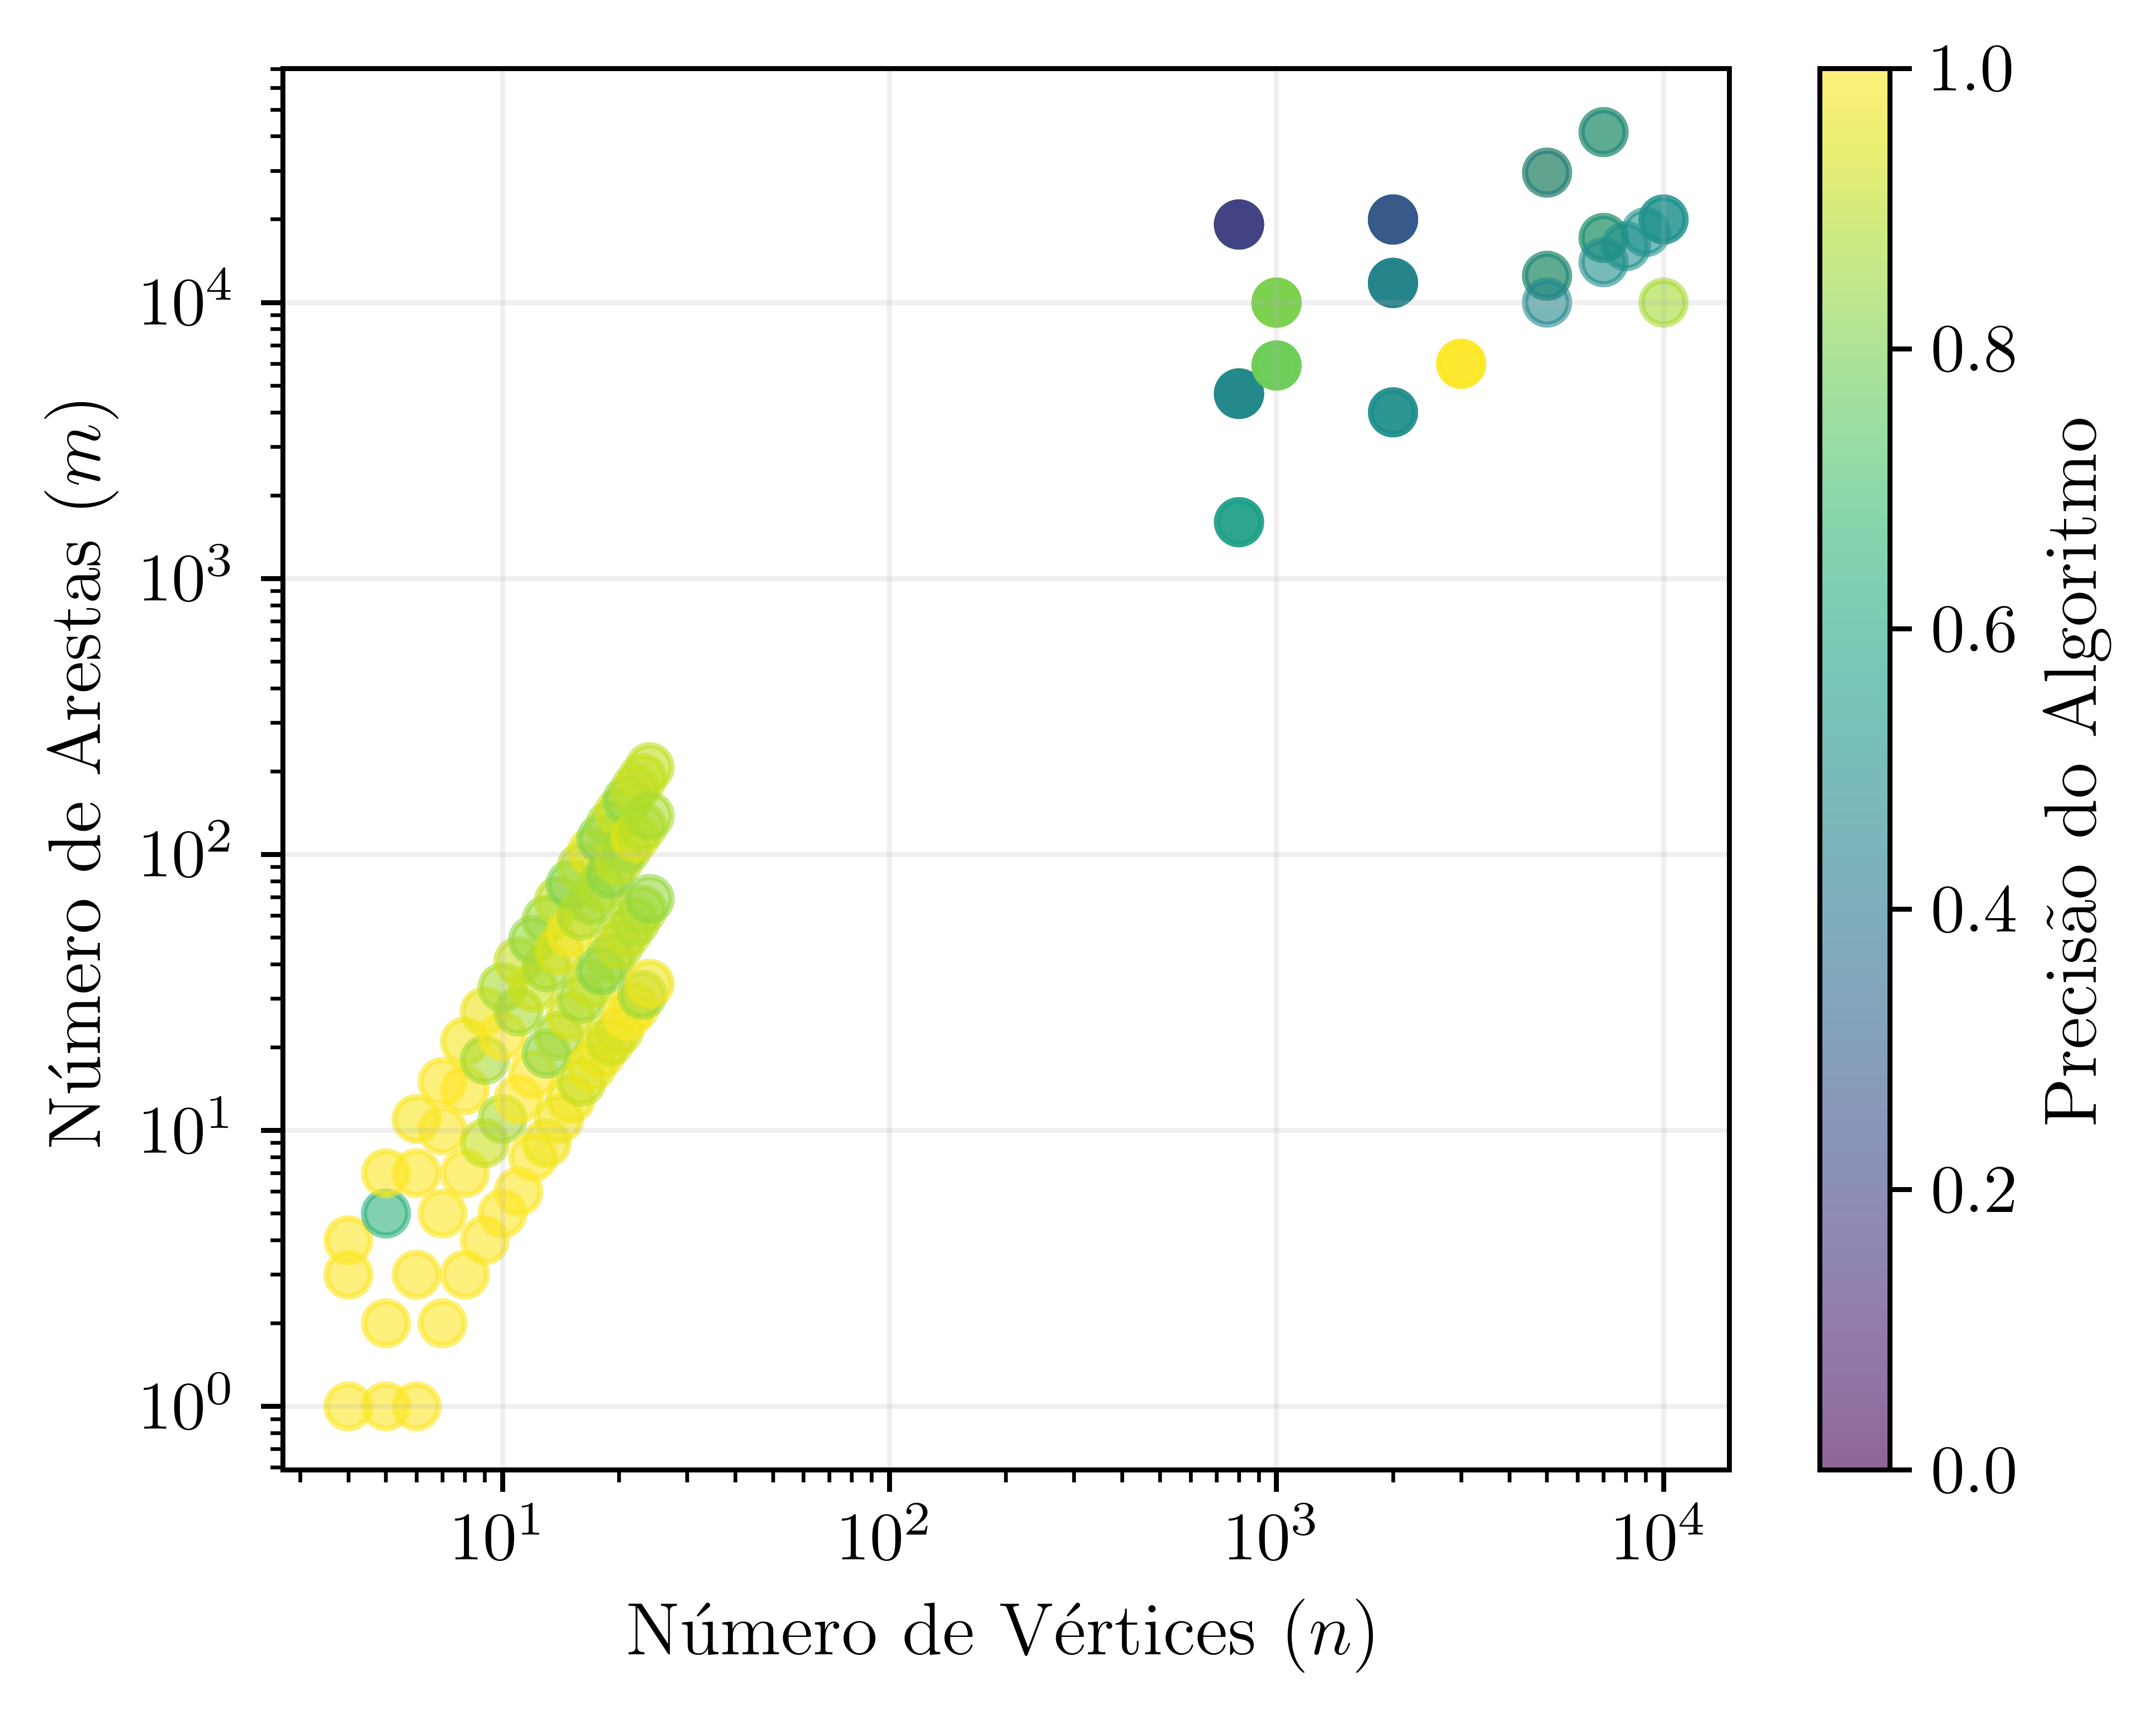
\includegraphics[width=0.4\textwidth]{../assets/precHEU.png}
    \caption{Precisão do algoritmo de heurística gulosa em função do número de vértices e de arestas.}
    \label{fig:precheu}
\end{figure}

Através da análise do gráfico, pode-se verificar que a precisão do algoritmo de heurística gulosa é influenciada pelo número de vértices e de arestas. Isto deve-se ao facto de que, quanto maior for o grafo, em termos de arestas, mais decisões locais o algoritmo terá de tomar, aumentando a probabilidade de fugir ao ótimo do problema, uma vez que as escolhas locais podem não ser as mais adequadas para o corte global. Para além disso, o número de vértices ao estar diretamente relacionado com o número de arestas, também revela uma influência na precisão.

Por fim, também foi calculada a média da precisão obtida para os grafos testados, sendo esta de aproximadamente $0.788$, revelando a capacidade do algortimo fornecer soluções de qualidade aceitável, especialmente para grafos de menor dimensão. Contudo, esta medida não deverá ser generalizada, visto que os grafos de menores dimensão ($n \leq 24$) foram testados em maior peso, face aos de maiores dimensões (\textit{Gset}).

\section{Conclusão}

Em suma, pode-se verificar, que existem várias abordagens para a resolução do problema do \textit{Maximum Weight Cut}, entre elas a pesquisa exaustiva e a heurística gulosa, cada qual com as suas vantagens e desvantagens.

Através da análise dos resultados obtidos com a aplicação destas abordagens, nota-se que o algortimo de pesquisa exaustiva, face à heurística gulosa, tem uma complexidade computacional que aumenta muito mais rapidamente com o número de vértices, em particular, de forma exponencial, enquanto que a heurística gulosa apresenta uma complexidade quadrática, revelando-se mais eficiente para grafos de maior dimensão.

Apesar do algortimo de heurística gulosa ter em seu favor a eficiência, como referido, este não garante a obtenção da solução ótima, pelo que a sua precisão varia de acordo com o grafo em análise, em contrapartida, o algoritmo de pesquisa exaustiva garante a obtenção da solução ótima, pelo que há um compromisso associado à escolha do algoritmo a ser aplicado. Ainda assim, foi possível observar que a heurística gulosa é capaz de fornecer soluções relativamente próximas à ótima, para grafos de menores dimensões, mas perdendo alguma precisão com o aumento do número de arestas.

Por fim, este estudo destacou a importância da escolha de abordagens metodológicas na resolução do problema do \textit{Maximum Weight Cut}, enfatizando como as características de cada algortimo influenciam tanto a qualidade das soluções como a eficiência do processo de resolução. Para além disso, embora apenas terem sido aplicados algoritmos determinísticos ao longo deste estudo, é provável que a integração de componentes estocásticas ou até mesmo a aplicação de técnicas de otimização via aprendizagem automática para ajustar as regras heurísticas, possam melhorar os resultados obtidos.

\bibliography{refs}

\end{document}
